%=======================02-713 LaTeX template, following the 15-210 template==================
%
% You don't need to use LaTeX or this template, but you must turn your homework in as
% a typeset PDF somehow.
%
% How to use:
%    1. Update your information in section "A" below
%    2. Write your answers in section "B" below. Precede answers for all 
%       parts of a question with the command "\question{n}{desc}" where n is
%       the question number and "desc" is a short, one-line description of 
%       the problem. There is no need to restate the problem.
%    3. If a question has multiple parts, precede the answer to part x with the
%       command "\part{x}".
%    4. If a problem asks you to design an algorithm, use the commands
%       \algorithm, \correctness, \runtime to precede your discussion of the 
%       description of the algorithm, its correctness, and its running time, respectively.
%    5. You can include graphics by using the command \includegraphics{FILENAME}
%
\documentclass[11pt]{article}
\usepackage{amsmath,amssymb,amsthm}
\usepackage{graphicx}
\usepackage[margin=1in]{geometry}
\usepackage{fancyhdr}
\usepackage{listings}
\usepackage{float}
\usepackage{subfig}

\setlength{\parindent}{0pt}
\setlength{\parskip}{5pt plus 1pt}
\setlength{\headheight}{13.6pt}
\newcommand\question[2]{\vspace{.25in}\hrule\textbf{#1: #2}\vspace{.5em}\hrule\vspace{.10in}}
\renewcommand\part[1]{\vspace{.10in}\textbf{(#1)}}
\newcommand\algorithm{\vspace{.10in}\textbf{Algorithm: }}
\newcommand\ot{\vspace{.10in}\textbf{Perform Model Selectio and Optimize: }}
\newcommand\pd{\vspace{.10in}\textbf{Process Data: }}
\newcommand\runtime{\vspace{.10in}\textbf{Compare Results: }}
\pagestyle{fancyplain}
\lhead{\textbf{\NAME\ (\ANDREWID)}}
\chead{\textbf{Final\HWNUM}}
\rhead{\today}
\begin{document}\raggedright
%Section A==============Change the values below to match your information==================
\newcommand\NAME{Yao Xiao}  % your name
\newcommand\ANDREWID{2019180015}     % your andrew id
\newcommand\HWNUM{}              % the homework number
%Section B==============Put your answers to the questions below here=======================

% no need to restate the problem --- the graders know which problem is which,
% but replacing "The First Problem" with a short phrase will help you remember
% which problem this is when you read over your homeworks to study.

\question{1}{Main Work} 

\part{a} \pd

The first is to read the data and analyze:

\begin{figure}[H]
    \centering
    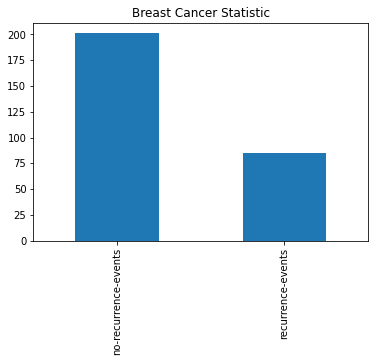
\includegraphics[width=0.6\textwidth]{Fig1}
    \caption{Breast Cancer Statistic}
\end{figure}

It is analyzed from Figure 1 that this is an unbalanced data set, which needs to be paid attention to when processing data.\\
Then analyze each group of feature data and find that some data are missing, and some features are not convenient for classification processing.

\begin{figure}[H]
    \centering
    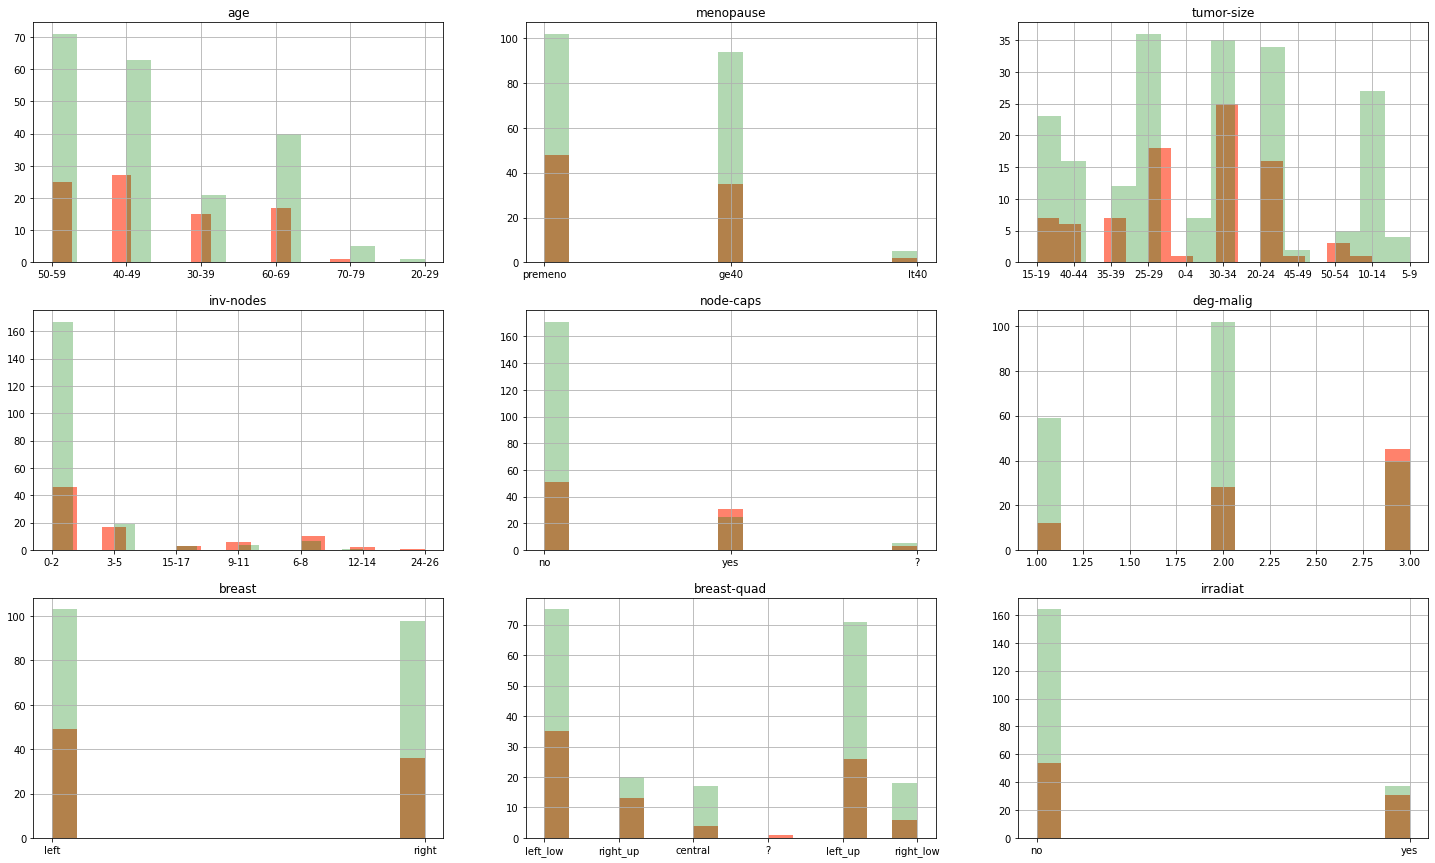
\includegraphics[width=1\textwidth]{Fig2}
    \caption{Visualize Data}
\end{figure}

Subsequent feature processing to facilitate classification, the main steps include but are not limited to binarize Class \& node-caps \& irradiat ; 
binarize Class \& node-caps \& irradiat; convert inv-nodes to the median of data; convert age to the numerical average of data; convert tumor-size to the numerical average of data. 
The results after processing are as follows:
\begin{figure}[H]
    \centering
    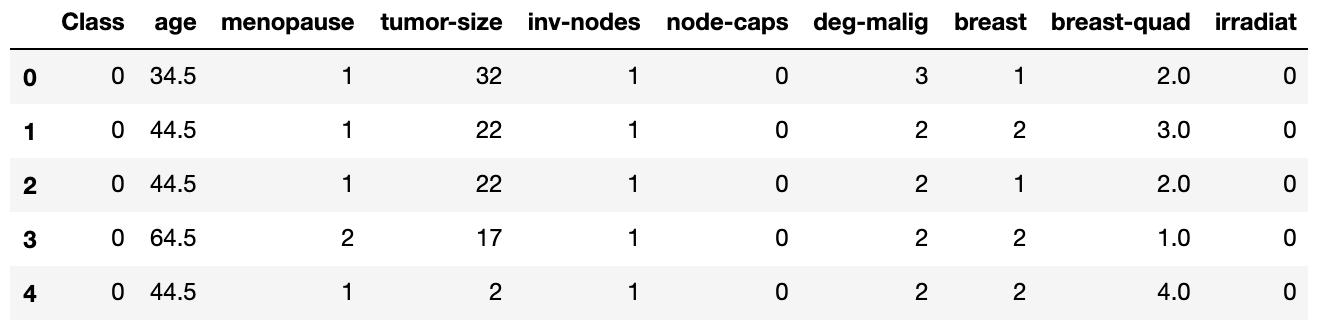
\includegraphics[width=1\textwidth]{Fig8}
    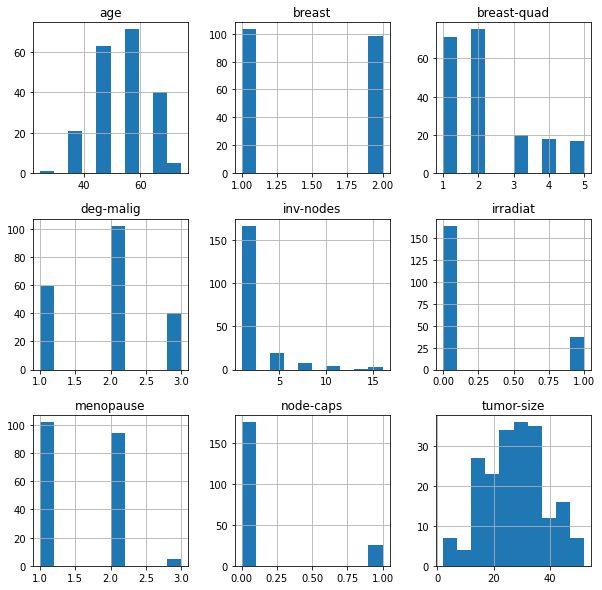
\includegraphics[width=1\textwidth]{Fig3}
    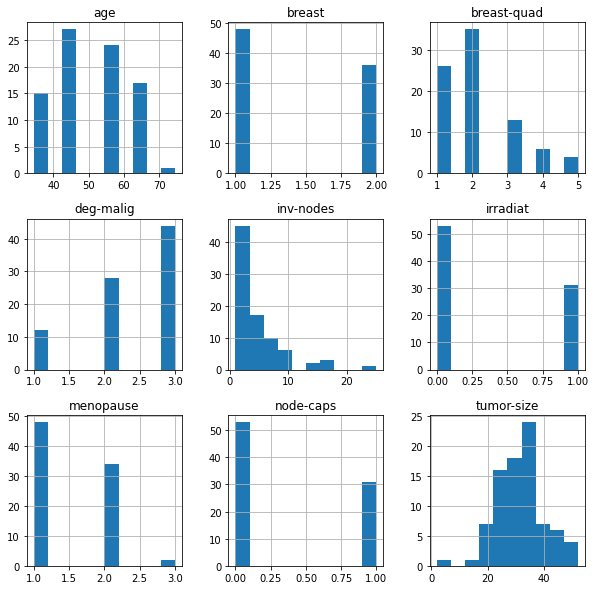
\includegraphics[width=1\textwidth]{Fig4}
    \caption{Processed Data}
\end{figure}

Also use randomforeast to analyze top features:
\begin{figure}[H]
    \centering
    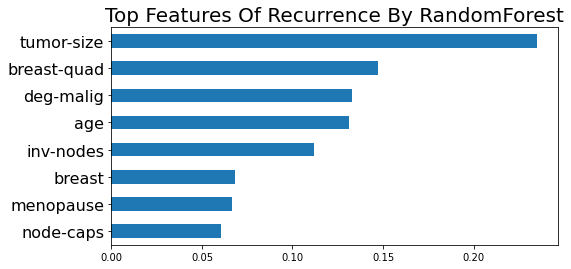
\includegraphics[width=1\textwidth]{Fig5}
    \caption{Top Features}
\end{figure}

\textbf{At last}, it can be analyzed from Figures 2, 3, and 4 that through filtering, 6 features relationships are retained --- ['age','menopause','tumor-size','inv-nodes','node-caps','deg-malig'].


\part{b} \ot

First split data to 70:30 ratio, and use StratifiedKFold for imbalance class. I selected three models of LogisticRegression, DecisionTree, GaussianNB to train, and evaluated from 6 dimensions such as recall rate.
\begin{figure}[H]
    \centering
    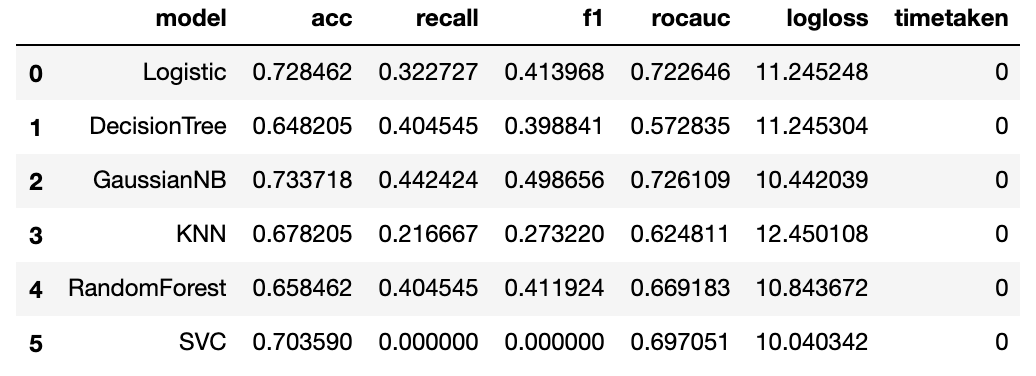
\includegraphics[width=1\textwidth]{Fig9}
    \caption{Output}
\end{figure}

And then optimise model: hyperparameter tuning
\begin{figure}[H]
    \centering
    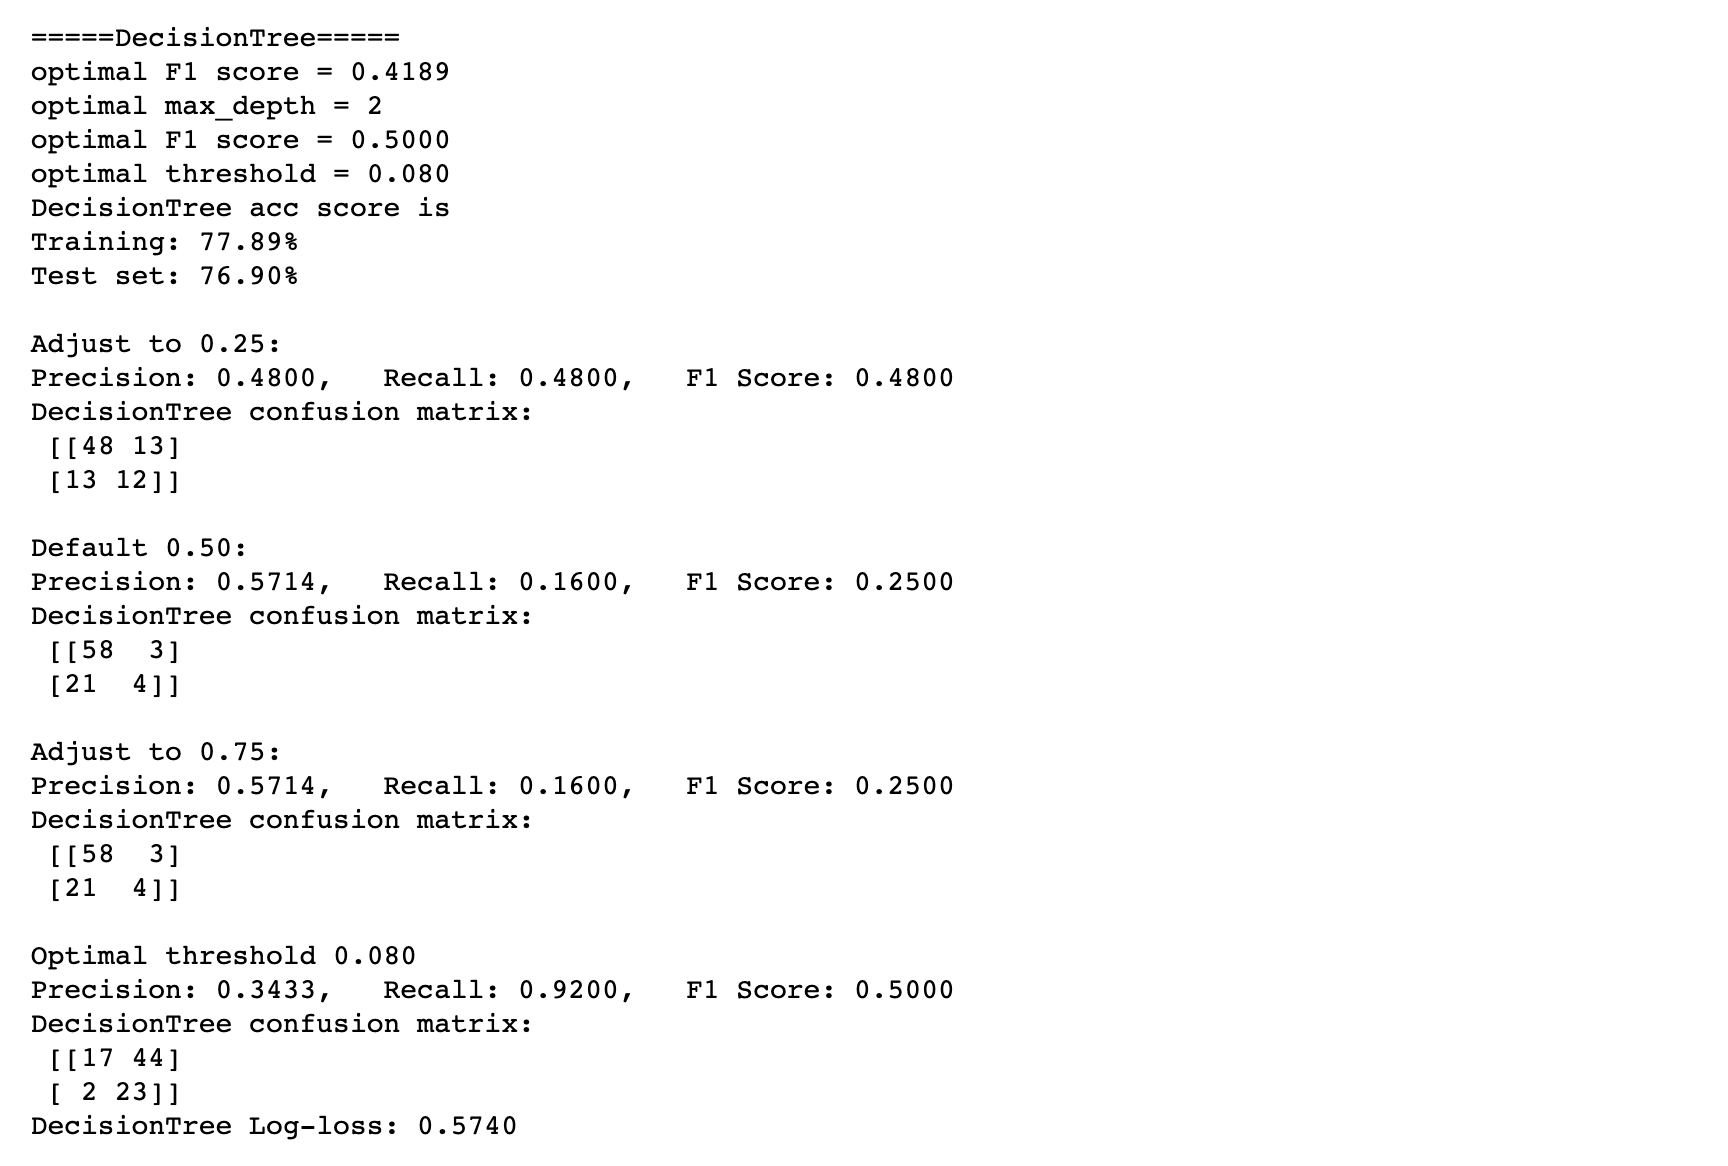
\includegraphics[width=1\textwidth]{Fig11}
    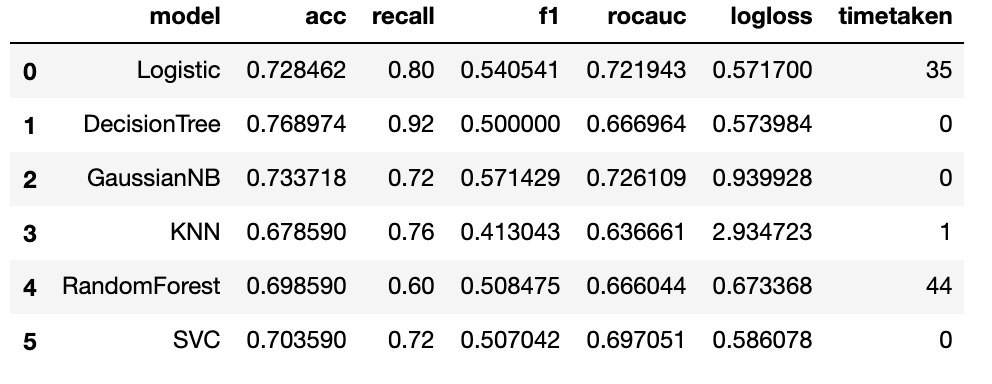
\includegraphics[width=1\textwidth]{Fig10}
    \caption{Optimized Output}
\end{figure}

\part{c} \runtime
After the comparison and optimization, the three models have achieved better results than before, and each evaluation dimension has been improved accordingly.
\textbf{At the same time, the best model should be DT}

\begin{figure}[H]
    \centering
    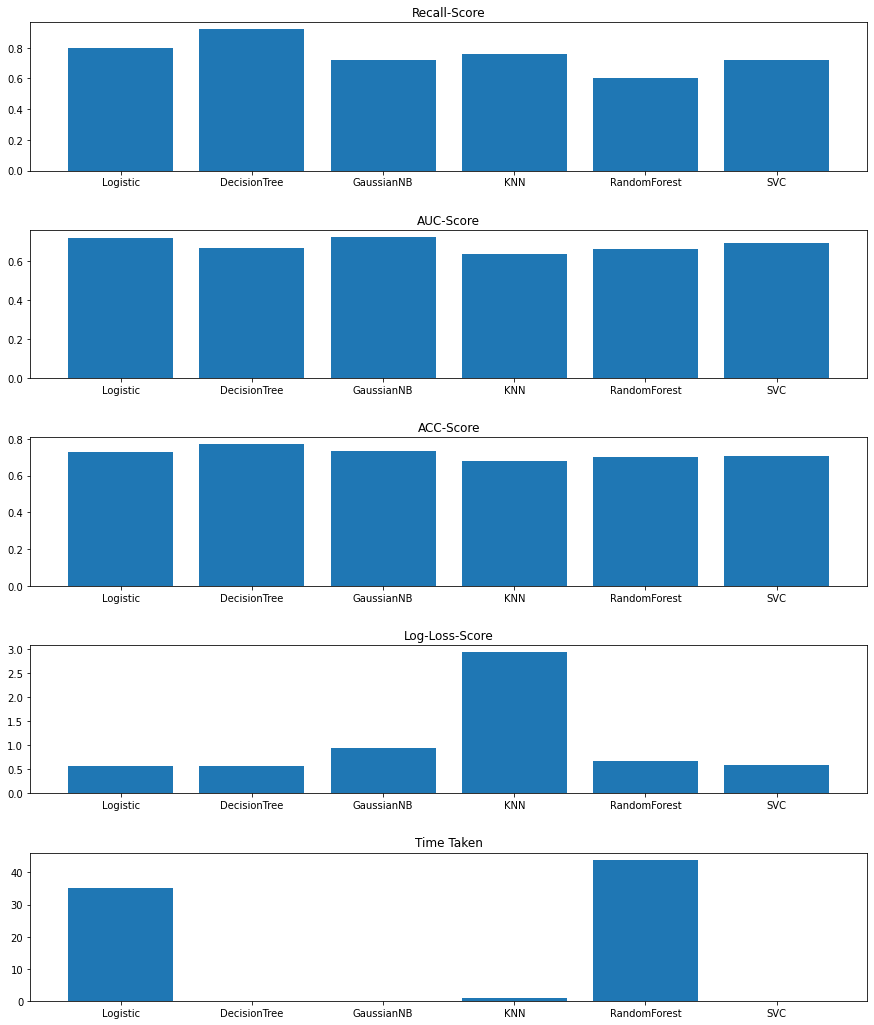
\includegraphics[width=0.6\textwidth]{Fig6}
    \caption{Evalute Result}
    \label{}
\end{figure}

\question{2}{Related Theory}
\vspace{.10in}\textbf{Logistic Regression:}
The core of the regression method is to find the most suitable parameters for the function, so that the value of the function is closest to the value of the sample. 
For example, linear regression is to find the most suitable a and b for the function f (x) = ax + b.

LR does not fit a linear function. It fits a function in probability. The value of f (x) now reflects the probability that the sample belongs to this class.

Applicable scenarios:

LR is also the basic component of many classification algorithms. Its advantage is that the output value naturally falls between 0 and 1 and has a probabilistic significance.

Because it is essentially a linear classifier, it cannot handle the correlation between features.

\vspace{.10in}\textbf{Decision Tree:}
The characteristic of a decision tree is that it is always segmenting along features. 
As the layers progress, this division will become more and more fine.

Although the generated tree is not easy for the user to see, when analyzing the data, by observing the upper structure of the tree, you can have an intuitive experience of the core idea of ​​the classifier.

Applicable scenarios:

Because it can generate a clear tree structure that selects different prediction results based on features, data analysts often use decision trees when they want to better understand the data at hand.

\vspace{.10in}\textbf{GaussianNB:}
In all machine learning classification algorithms, Naive Bayes is different from most other classification algorithms. 
For most classification algorithms, such as decision trees, KNN, logistic regression, support vector machines, etc., they are all discriminant methods, that is, directly learning the relationship between the feature output Y and the feature X, or the decision function Y = f 
(X), or the conditional distribution P (Y | X). 
However, Naive Bayes is a generation method, that is, to directly find the joint distribution P (X, Y) of the feature output Y and the feature X, and then use P(Y) inferred.

Applicable scenarios:

GaussianNB is generally used to process sample features, most of which are continuous values.


Based on the above foundation, the optimization method is searching for optimal threshold, vary from 0.0001 to 0.9999, fit/predict on train/test data.

\begin{enumerate}
    \item Search for optimal hyperparameter C in LogisticRegresssion, vary C from 0.001 to 1000, using KFold(5) Cross Validation on train data.
    \item Search for optimal max depth in DecisionTree, vary 2 to 10, using KFold(8) cross validation on train data
\end{enumerate}

\begin{lstlisting}
print('\n=====LogisticRegression=====')
time1 = time.time()
kf = KFold(n_splits=5, random_state=SEED, shuffle=True)  
score_list = []
c_list = 10**np.linspace(-3,3,300)
for c in c_list:
    logit = LogisticRegression(C = c)
    cvs = (cross_val_score(logit,x_train, y_train, cv=kf, scoring='f1')).mean()
    score_list.append(cvs)
print('optimal cv F1 score = {:.4f}'.format(max(score_list)))
optimal_c = float(c_list[score_list.index(max(score_list))])
print('optimal value of C = {:.3f}'.format(optimal_c))

logic = LogisticRegression(C = optimal_c)
model1 = optimise_record(logic, x_train, x_test, y_train, y_test, 'Logistic')
model1.timetaken[0] = time.time() - time1

print('\n=====DecisionTree=====')
time1 = time.time()
kf = KFold(n_splits=8, random_state=SEED, shuffle=True)
d_scores = []
for d in range(2, 11):
    decisiontree = DecisionTreeClassifier(max_depth=d)
    cvs = cross_val_score(decisiontree, x_train, y_train, cv=kf, scoring='f1').mean()
    d_scores.append(cvs)
print('optimal F1 score = {:.4f}'.format(max(d_scores)))   
optimal_d = d_scores.index(max(d_scores))+2   
print('optimal max_depth =', optimal_d)

decisiontree = DecisionTreeClassifier(max_depth=optimal_d)
model2 = optimise_record(decisiontree, x_train, x_test, y_train, y_test, 'DecisionTree')
model2.timetaken[0] = time.time() - time1

print('\n=====GaussianNB=====')
time1 = time.time()
gnb = GaussianNB()
model3 = optimise_record(gnb, x_train, x_test, y_train, y_test, 'GaussianNB')
model3.timetaken[0] = time.time() - time1
\end{lstlisting}



\question{3}{Some Comments}
The data of this project is relatively easy to handle. It should be noted that the data should also be normalized when processing the data. For the data of the range category, it is better to use the median to replace it for further classification.

Because the features are clear, DT may achieve better results.In fact, each model has achieved good results, but considering that this is an extremely imbalance data set, we should focus on the recall rate rather than the accuracy rate, so the best model is DecisionTree, and DT is still achieved gratifying resultson other data.
At the same time, DT has achieved good results in acc, auc, loss, and timetaken.

\begin{figure}[H]
    \centering
    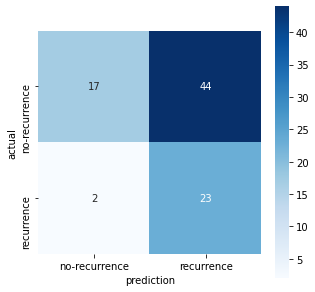
\includegraphics{Fig7}
    \caption{DT Confusion Matrix}
\end{figure}
\end{document}
